\documentclass[11pt]{article}

%% MinionPro fonts 
%\usepackage[lf]{MinionPro}
%\usepackage{MnSymbol}
\usepackage{microtype}

%% Margins
\usepackage{geometry}
\geometry{verbose,letterpaper,tmargin=1in,bmargin=1in,lmargin=1in,rmargin=1in}

%% Other packages
\usepackage{amsmath}
\usepackage{amsthm}
\usepackage[shortlabels]{enumitem}
\usepackage{titlesec}
\usepackage{soul}
\usepackage{tikz}
\usepackage{mathtools}
\usepackage{pgfplots}
\usepackage{tikz-3dplot}
\usepackage{algorithmic}
\usepackage[export]{adjustbox}
\usepackage{tcolorbox}
\usepackage{mathrsfs}
\usepackage{optprog}

%% Paragraph style settings
\setlength{\parskip}{\medskipamount}
\setlength{\parindent}{0pt}

%% Change itemize bullets
\renewcommand{\labelitemi}{$\bullet$}
\renewcommand{\labelitemii}{$\circ$}
\renewcommand{\labelitemiii}{$\diamond$}
\renewcommand{\labelitemiv}{$\cdot$}

%% Colors
\definecolor{rred}{RGB}{204,0,0}
\definecolor{ggreen}{RGB}{0,145,0}
\definecolor{yyellow}{RGB}{255,185,0}
\definecolor{bblue}{rgb}{0.2,0.2,0.7}
\definecolor{ggray}{RGB}{190,190,190}
\definecolor{ppurple}{RGB}{160,32,240}
\definecolor{oorange}{RGB}{255,165,0}

%% Shrink section fonts
\titleformat*{\section}{\normalsize\bf}
\titleformat*{\subsection}{\normalsize\bf}
\titleformat*{\subsubsection}{\normalsize\it}

% %% Compress the spacing around section titles
\titlespacing*{\section}{0pt}{1.5ex}{0.75ex}
\titlespacing*{\subsection}{0pt}{1ex}{0.5ex}
\titlespacing*{\subsubsection}{0pt}{1ex}{0.5ex}

%% amsthm settings
\theoremstyle{definition}
\newtheorem{problem}{Problem}
\newtheorem{example}{Example}
\newtheorem*{theorem}{Theorem}
\newtheorem*{bigthm}{Big Theorem}
\newtheorem*{biggerthm}{Bigger Theorem}
\newtheorem*{bigcor1}{Big Corollary 1}
\newtheorem*{bigcor2}{Big Corollary 2}

%% tikz settings
\usetikzlibrary{calc}
\usetikzlibrary{patterns}
\usetikzlibrary{decorations}
\usepgfplotslibrary{polar}

%% algorithmic setup
\algsetup{linenodelimiter=}
\renewcommand{\algorithmiccomment}[1]{\quad// #1}
\renewcommand{\algorithmicrequire}{\emph{Input:}}
\renewcommand{\algorithmicensure}{\emph{Output:}}

%% Answer box macros
%% \answerbox{alignment}{width}{height}
\newcommand{\answerbox}[3]{%
  \fbox{%
    \begin{minipage}[#1]{#2}
      \hfill\vspace{#3}
    \end{minipage}
  }
}

%% \answerboxfull{alignment}{height}
\newcommand{\answerboxfull}[2]{%
  \answerbox{#1}{6.38in}{#2} 
}

%% \answerboxone{alignment}{height} -- for first-level bullet
\newcommand{\answerboxone}[2]{%
  \answerbox{#1}{6.0in}{#2} 
}

%% \answerboxtwo{alignment}{height} -- for second-level bullet
\newcommand{\answerboxtwo}[2]{%
  \answerbox{#1}{5.8in}{#2}
}

%% special boxes
\newcommand{\wordbox}{\answerbox{c}{1.2in}{.7cm}}
\newcommand{\catbox}{\answerbox{c}{.5in}{.7cm}}
\newcommand{\letterbox}{\answerbox{c}{.7cm}{.7cm}}

%% Miscellaneous macros
\newcommand{\tstack}[1]{\begin{multlined}[t] #1 \end{multlined}}
\newcommand{\cstack}[1]{\begin{multlined}[c] #1 \end{multlined}}
\newcommand{\ccite}[1]{\only<presentation>{{\scriptsize\color{gray} #1}}\only<article>{{\small [#1]}}}
\newcommand{\grad}{\nabla}
\newcommand{\ra}{\ensuremath{\rightarrow}~}
\newcommand{\maximize}{\text{maximize}}
\newcommand{\minimize}{\text{minimize}}
\newcommand{\subjectto}{\text{subject to}}
\newcommand{\trans}{\mathsf{T}}
\newcommand{\bb}{\mathbf{b}}
\newcommand{\bx}{\mathbf{x}}
\newcommand{\bc}{\mathbf{c}}
\newcommand{\bd}{\mathbf{d}}

%% LP format
%    \begin{align*}
%      \maximize \quad & \mathbf{c}^{\trans} \mathbf{x}\\
%      \subjectto \quad & A \mathbf{x} = \mathbf{b}\\
%                       & \mathbf{x} \ge \mathbf{0}
%    \end{align*}


%% Redefine maketitle
\makeatletter
\renewcommand{\maketitle}{
  \noindent SA405 -- AMP \hfill Rader \S 4.1--page 126 \\

  \begin{center}\Large{\textbf{\@title}}\end{center}
}
\makeatother

%% ----- Begin document ----- %%
\begin{document}
  
\title{Lesson 12.  Vehicle Routing Problem (VRP)}

\maketitle

%%%
\section{This lesson}

\begin{itemize}
	\item  Description of the Vehicle Routing Problem
	\item  Pizza Delivery Example
	\item  Generalized subtour elimination constraints
	\item  The ``final'' VRP model
\end{itemize}

\section{VRP:  An extension of TSP}

\textbf{Vehicle Routing Problems} are similar to TSP, except that instead of having a single ``salesperson'', we have multiple ``salespeople'' (vehicles), all \emph{starting and ending at the same location}.  We must decide the ``cheapest'' way to cover all of the locations via tours with our fleet of salespeople.

\begin{problem} The pizza restaurant at {\huge ${\star}$} has 12 delivery orders ready and three drivers.  Each driver can serve at most 5 customers.  Draw a \emph{feasible} solution to the VRP problem on the graph below.

\vspace{-.5cm}
\begin{center}
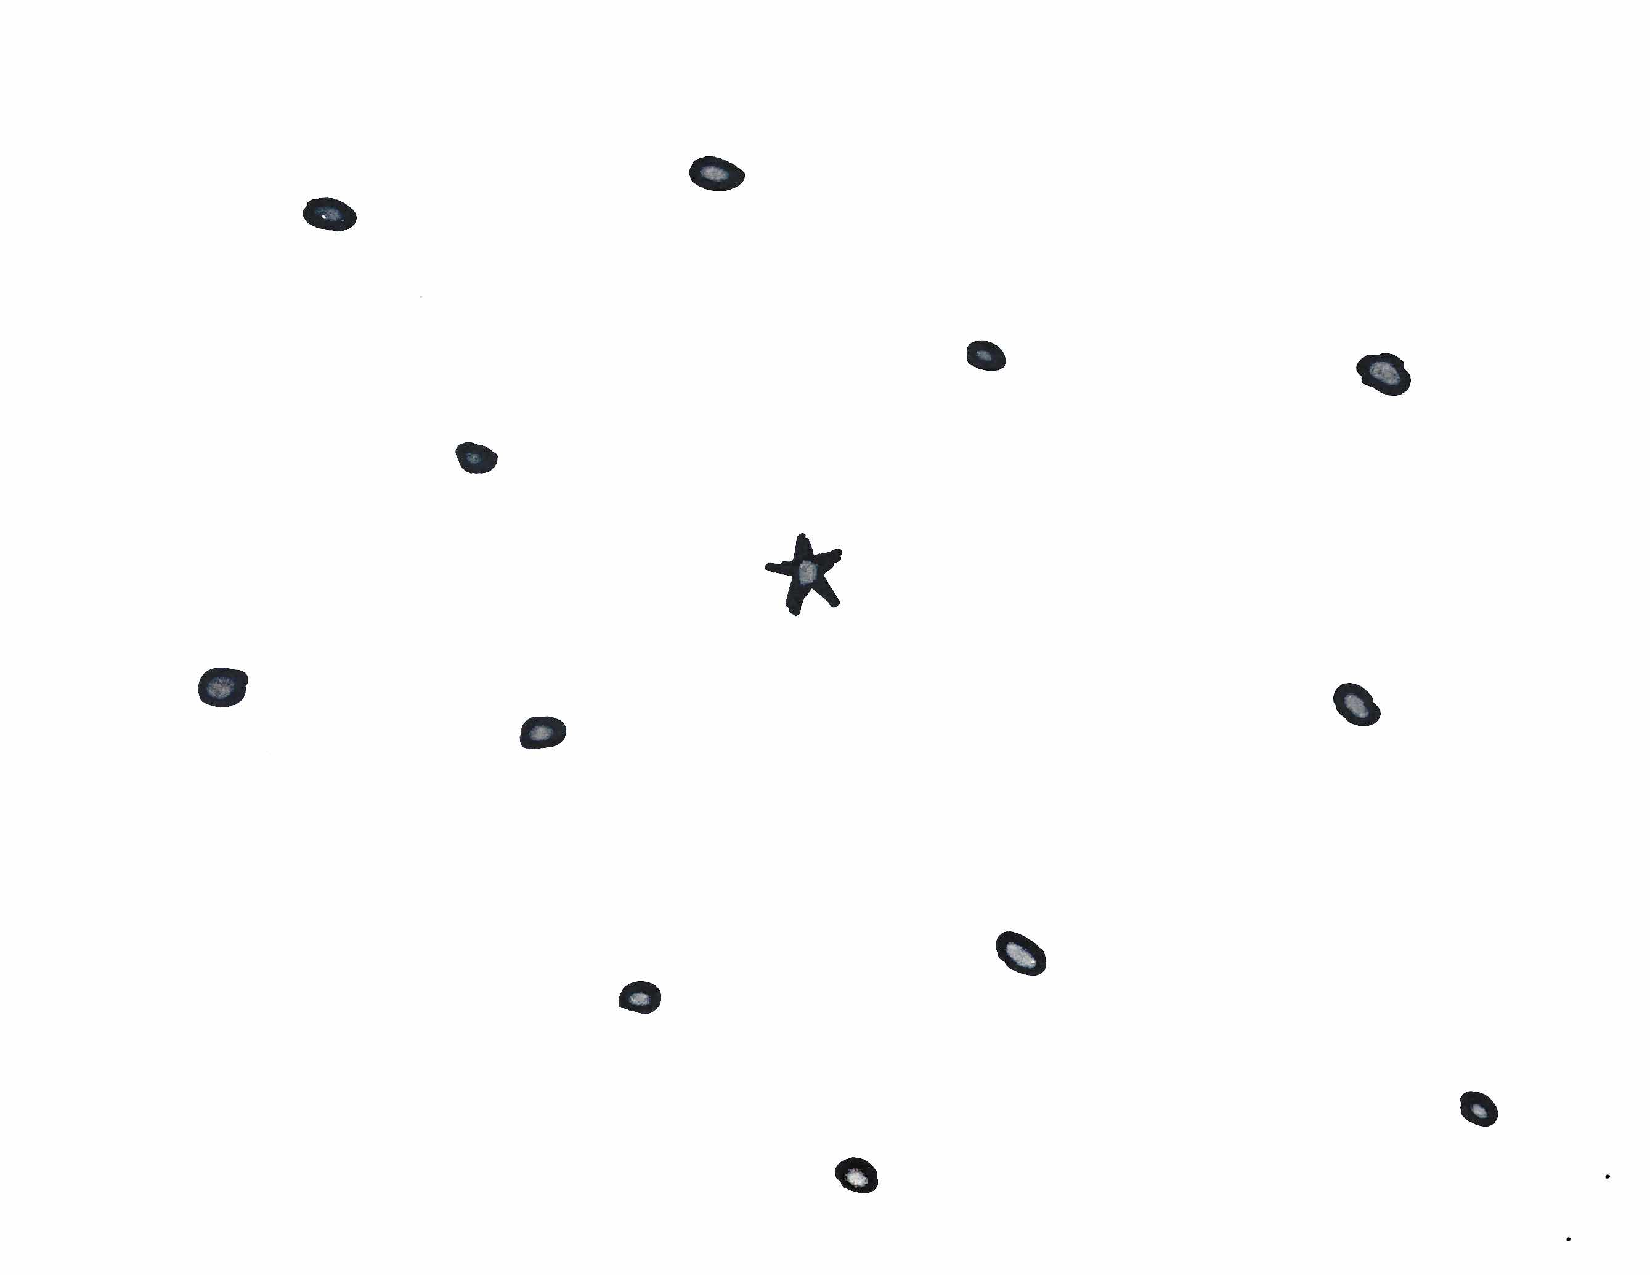
\includegraphics[width=0.5\textwidth]{pizza}
\end{center}
\end{problem}

\bigskip
\begin{tcolorbox}
Vehicle routing is a very practical real world application.
\end{tcolorbox}



\newpage

\textbf{Basic VRP}
\begin{itemize}
	\item Fixed number of vehicles.
	\item All vehicles start and end a common location, or \textbf{depot}.
	\item All vehicles have the same capacity.  
	\item Vehicles may serve many different customers, up to capacity.
	\item Each customer's demand must be served by a single vehicle.
	\item Goal:  Find a minimum cost collection of \emph{tours}, all starting and ending at the depot, that contain all customers and do not violate vehicle capacities.
\end{itemize}




\begin{tcolorbox}
\textbf{Basic VRP:  Mathematical Description}

Notation: 
\begin{itemize}
	\item Let $G = (N,E)$ be an undirected graph.  
		\begin{itemize}
			\item One of the nodes is distinguished as the \emph{depot}: usually vertex ``$0$''.
			\item Each edge has a cost (or distance): $c_{ij},$ for $(i,j) \in E$ Remember that $(i,j) \in E$ if $i < j$.
			\item Each node has a demand: $d_i$, for $i \in N$.
		\end{itemize}
	\item  Exactly $k$ tours (vehicles) used, each with the same demand capacity ($D$).
\end{itemize}

Requirements:
\begin{itemize}
	\item Each tour must include the depot.
	\item Each vertex (customer) must be be served.
	\item The demand of each tour must not exceed D.
\end{itemize}

Formulation assumptions:
\begin{itemize}
	\item Every vehicle visits at least two customers.
	\item The direction an edge is traversed does not affect the cost.
	\item (Variations of the formulation can work around these assumptions.)
\end{itemize}
Goal:
\begin{itemize}
	\item  Minimize total cost of tours.
\end{itemize}
\end{tcolorbox}


VRP can be modified to incorporate variations including:
\begin{itemize}
\item \textbf{Capacitated VRP:} Each vehicle has a capacity (problem we are doing)
\item \textbf{VRP with time windows:}  Each customer must be visited within a certain time window
\item \textbf{Multidepot VRP:}  Fixed number of vehicles starting at each of multiple depots. 
\item \textbf{Split delivery VRP: } Customer demand can be met by more than one vehicle
\end{itemize}

\newpage

\section{VRP Standard Formulation: Pizza Deliveries (Example 4.1 in Rader, page 127)}

\begin{problem}
A local pizza shop received 10 orders for delivery last night with three delivery persons working.  The shop uses a coordinate system to
mark where houses are located (using the nearest intersection as locations).  The
10 deliveries are to go to the following places:

\begin{center}
\begin{tabular}{|c|c|c|c|c|c|c|c|c|c|c|}
\hline
& 1 & 2 & 3 & 4 & 5 & 6 & 7 & 8 & 9 & 10  \\
\hline
E/W & 20 & 40 & 180 & 130 & 160 & 40 & 30 & 100 & 90 & 75 \\
\hline
N/S & 90 & 70 & 20 & 100 & 10 & 80 & 50 & 60 & 120 & 15 \\
\hline
\end{tabular}
\end{center}

All streets in town go either north-south or east-west, so distance must be
measured rectilinearly.  Assuming that the pizza shop is located at position (0,0)
and that each driver can deliver at most five orders, how should the delivery
routes be determined to minimize the total travel distance? 
\end{problem}

\begin{enumerate}
\item Write an abbreviated concrete model to minimize the distance traveled by the pizza shop. Do \textbf{not} include subtour elimination constraints. \emph{Hint: there are two types of constraints, one for each node other than the depot and one for the depot.}
\end{enumerate}

\newpage

\begin{problem}
Suppose a solution to the (incomplete) model above  gives the following cycles: $\{0,2,4\}, \{0,6,9\}, \{0,8,10\}, \{1,3,5,7\}$.
	\begin{enumerate}
	\item[(a)] Sketch the graph associated with this solution. \vfill
	\item[(b)] What are the values of the edges corresponding to this solution? 
	\vfill
	\item[(c)] Why is this solution infeasible to the (complete) VRP formulation? 
	\vfill
	\item[(d)] Using the MST/TSP style, write a concrete constraint that would eliminate this solution from the feasible region. \vfill
	\end{enumerate}
\end{problem}

\newpage

\begin{problem}
Suppose a solution to the (incomplete) model above  gives the following cycles: $\{0,2,4\}, \{0,6,9\}, \{0,1,3,5,7,8,10\}$.
	\begin{enumerate}
	\item[(a)] Sketch the graph associated with this solution. \vfill
	\item[(b)] What are the values of the edges corresponding to this solution? 
	\vfill
	\item[(c)] Why is this solution infeasible to the (complete) VRP formulation? 
	\vfill
	\item[(d)] Write a concrete constraint that would eliminate this solution from the feasible region \emph{without including any edges connected to node 0 (we will see why soon)}.
	\end{enumerate}
\end{problem}
\vfill
\newpage

\section{Route Splitting in VRP}

The \textbf{subtour elimination constraints} that we learned about in MST and TSP would technically work for VRP but would make the solution process very difficult. Thus, prior to parameterizing the VRP problem; we introduce a new type of subtour elimination constraints called which work for the VRP (these are also the types of constraints you'll use for project 2!).

\begin{tcolorbox}
A \textbf{connected component} is a subset of nodes in a graph which are all connected to each other.
\end{tcolorbox}

The question we ask in VRP is: How many edges must we include among $|S|$ vertices in order to have $C$ connected components and NO CYCLES (importantly, this means you need $C$ vehicles to visit each of these customers)?  Let's try some test cases...

\begin{itemize}
\item $C = 1$: How many edges do we include to have 1 connected component and no cycles?
\begin{center}
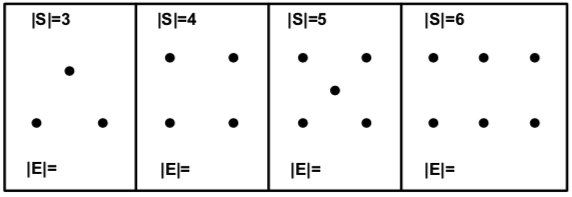
\includegraphics[width=0.75\textwidth]{four_graphs.png}
\end{center}
\item $C = 2$: How many edges do we include to have 2 connected components and no cycles?
\begin{center}
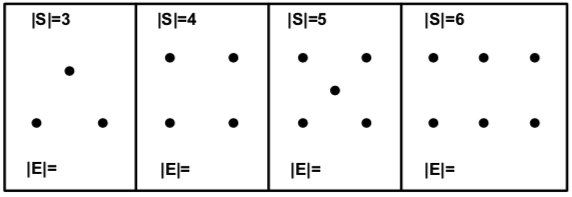
\includegraphics[width=0.75\textwidth]{four_graphs.png}
\end{center}
\item $C = 3$: How many edges do we include to have 3 connected components and no cycles?
\begin{center}
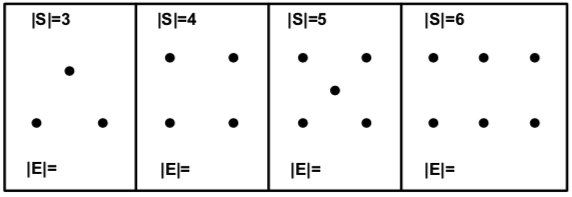
\includegraphics[width=0.75\textwidth]{four_graphs.png}
\end{center}
\end{itemize}

\newpage

Given a general $C > 0$, how many edges must we include among $|S|$ nodes to have $C$ connected components and no cycles? These are called \textbf{generalized subtour elimination} constraints.
\vspace{1in}

\section{Parameterized VRP Model}

\begin{problem}
Write the full parameterized VRP model using the generalized subtour elimination constraints.
\end{problem}




\end{document}

